\section{Method and Experimental Apparatus}
\subsection{Physical implementation}
The OV5647 camera, Raspberry Pi 3 B+ and LightRanger 14 Click (TMF8829) are fixed on a tripod. We retained the Lab~1 kit lens, with nominal focal length approximately 30\,mm. Tape holds the depth board above the camera, leaving its optical window clear. Two team-built guide edges constrain a sliding base carrying a printed USAF target in an existing upright stand (Fig.~\ref{fig:apparatus}). An ASUS ROG Strix XG27UCGR monitor (27-inch, native $3840\times2160$) illuminates the paper from the side. We checked that the selected depth zones saw the paper: placing the monitor in the ranging field had previously caused foreground returns.

\begin{figure*}[t]
\centering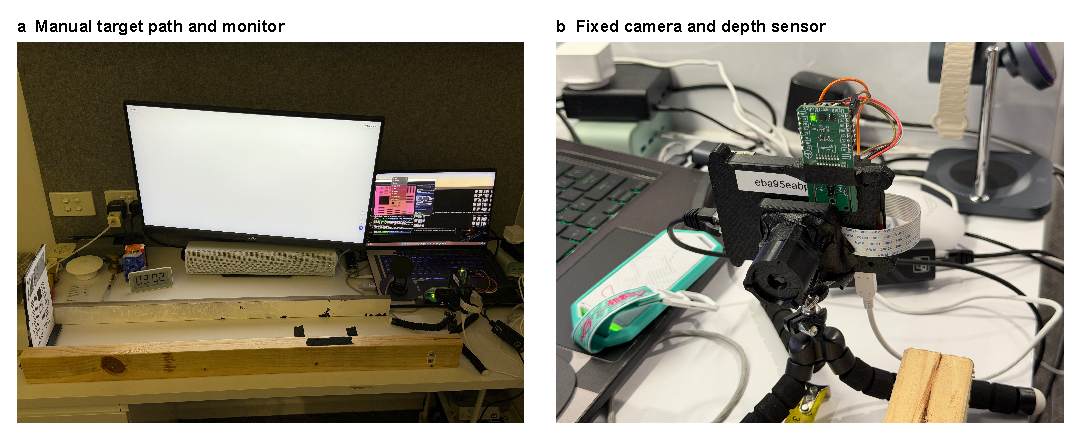
\includegraphics[width=\textwidth]{images/apparatus.pdf}
\caption{Apparatus used for the supplementary experiment. (a) Printed target, manual guide path, side monitor and fixed sensors. (b) Camera and depth board on the kit plate. The team built the guide; the upright target stand and kit plate were supplied. The photographs show placement; alignment and mounting stiffness were not measured.}
\label{fig:apparatus}
\end{figure*}

The base front moves from 75 to 65\,cm toward the camera. The paper lies 22\,mm behind it, giving $D_{\rm paper}=D_{\rm edge}+22$\,mm. This converts the position reference; it does not measure sensor bias because the ruler zero was not surveyed against the optical origin. We kept focus, aperture, monitor position and brightness fixed. The monitor was set to 160\,Hz and brightness-menu value 90; optical transition times and luminance were not measured independently.

\Needspace{10\baselineskip}
\subsection{Acquisition and independent repeats}
The dataset contains 40 runs and 1239 readable DNG images, covering calibration, stationary controls and 16 motion attempts. Twelve eligible independent pushes cover coded/steady-white illumination and smooth/variable push instructions, with three pushes in each cell. For variable pushes, the operator deliberately changed speed; for smooth pushes, the operator tried to keep the motion steady. Both instructions still allowed measured velocity to vary. We retained two pilots and two weak-motion originals outside the primary set, and collected extra independent pushes to replace the weak variable-motion attempts.

Each run saves repeated camera DNGs and continuous $8\times8$ depth arrays. Coded runs also save received illumination events. We select one exposure per push for the primary analysis, so multiple frames and zones do not count as independent trials. Exposure and analogue gain were requested at 1\,s and 1. Metadata give an exposure of 999942\,$\mu$s; actual gain was not independently checked. Acquisition is $640\times480$, reduced to $240\times180$ linear-green images for analysis.

The monitor repeats \texttt{1101001101} in nominal 200\,ms states, giving a 2\,s period and 60\% white duty cycle. We play the code for 12\,s within a 20\,s recording. The camera integrates throughout each exposure while the monitor changes the paper's illumination. Since one second covers only part of the code period, we use the state history logged for that exposure to calculate its weights. White and coded runs involve separate pushes, with unmatched trajectories and light dose.

\subsection{Exposure selection}
We fixed an exploratory selection rule before computing reconstruction scores, without preregistration. A primary exposure needs depth coverage, reliable event coverage for coded light, an approaching target and at least 15\,mm travel during integration. We reject windows crossing anomalous event intervals, then select the largest travel for smooth pushes or the largest departure from endpoint-linear depth for variable pushes. The two weak originals reach only 9.05 and 6.99\,mm maximum travel and are scored separately. One coded run has an event freeze after the selected window; its earlier covered window remains usable. Event counts alone would not reveal this problem.
